\documentclass[tikz,border=1mm]{standalone}
\usetikzlibrary{positioning}

\usepackage{xcolor}
\colorlet{myred}{red!80!black}
\colorlet{myblue}{blue!80!black}
\colorlet{mybluee}{myblue!80!black}
\colorlet{mygreen}{green!60!black}
\colorlet{myorange}{orange!70!red!60!black}
\colorlet{mydarkred}{red!30!black}
\colorlet{mydarkblue}{blue!40!black}
\colorlet{mydarkgreen}{green!30!black}

\begin{document}

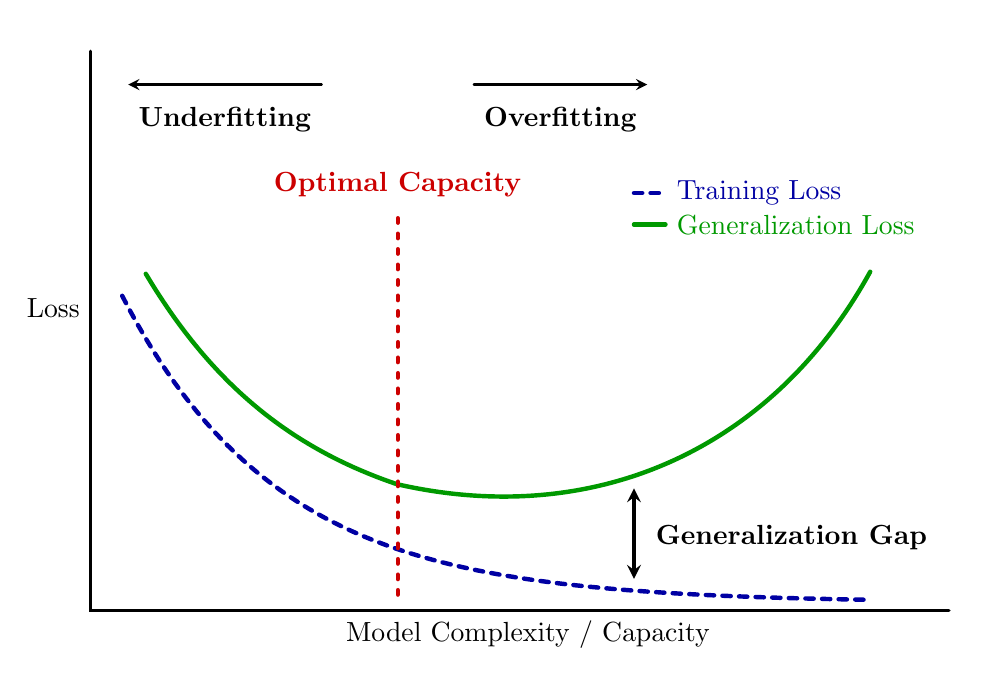
\begin{tikzpicture}[thick,line cap=round,>=stealth,node
    distance=1em]
    
\clip (-0.7,-0.7) rectangle + (12,8);

 % Training Loss
 % \draw[dashed, ultra thick, mybluee] (0.8,5) to[bend right=45] node[pos=0.7,above right] {}(4,0.5);
 % \draw[dashed, ultra thick, mybluee] (4,0.5) to[bend right=24] node[pos=0.7,above right] {}(30,7.8);
 \draw[dashed, ultra thick, mybluee, domain=0.5:10, samples=100] plot (\x, {5*exp(-0.5*\x)});
 \draw[draw=white, fill = white] (10,0) rectangle ++(4.3,1.3);

 % Generalization Loss
 \draw[ultra thick, mygreen] (4,1.5) to[bend right=37] node[pos=0.7,above right] {}(10,4.2);
 \draw[ultra thick, mygreen, domain=0.8:4, samples=100] plot (\x, {5*exp(-0.5*\x)+0.822});

  
 \draw[loosely dotted, ultra thick, myred] (4,0.1) -- (4,5) node[above] (P) {\textbf{Optimal Capacity}};
 
 \path node[above left=of P, xshift=1cm] (U) {\textbf{Underfitting}}
    node[above right=of P, xshift=-1cm] (O) {\textbf{Overfitting}};
    
 \draw[->] ([yshift=1ex]U.north east) -- ([yshift=1ex]U.north west);
 \draw[->] ([yshift=1ex]O.north west) -- ([yshift=1ex]O.north east);   

 \draw [-, very thick] (0.1,7) node[below left, yshift=-3cm]{Loss} |- (11,-0.1) node[below left, xshift=-2.9cm]{Model Complexity / Capacity};

  \draw[<->, very thick] (7,1.45) -- (7,0.3);

  \node at (9,0.83) {\textbf{Generalization Gap}};


  % Legend
  \draw[dashed, ultra thick, mybluee] (7,5.2) -- (7.4,5.2) node[right] {Training Loss};
  \draw[ultra thick, mygreen] (7,4.8) -- (7.4,4.8) node[right] {Generalization Loss};

\end{tikzpicture}

\end{document}